\section{Introduction to Stellarium}
\label{app:stell}
\newcommand{\stellarium}{\textit{Stellarium}}
\newcommand{\icon}[1]{\includegraphics[height=0.2in]{appendices/stellarium/stell-#1.pdf}}

\bigskip\bigskip

\stellarium\ is a software application that simulates the appearance
of astronomical objects in the sky. The user can adjust lots of
features of the view, including the observer's location,
the time, etc. We may not use it all that much this semester,
because we'll be using the \textit{Sky Safari$+$} app on the iPads
instead, but \textit{Stellarium} is more powerful than
\textit{Sky Safari$+$}, so we'll use it on occasion.

\stellarium\ is free. I encourage you to download it onto your own computer
by going to {\tt http://stellarium.org},
so that you can play with it outside of class. You may find it helpful when 
studying or answering homework questions.

In this Appendix, I'll list some of the features of the program that will
be most useful to us. The best way to learn about these features is not
just to read about them here, though. Spend some time playing around, to learn
what you can do.

Many of the useful features in \stellarium\ are in two menus that pop up
on the bottom left of the screen when you move the mouse over to
that region:

\begin{center}
\vspace{0.1in}
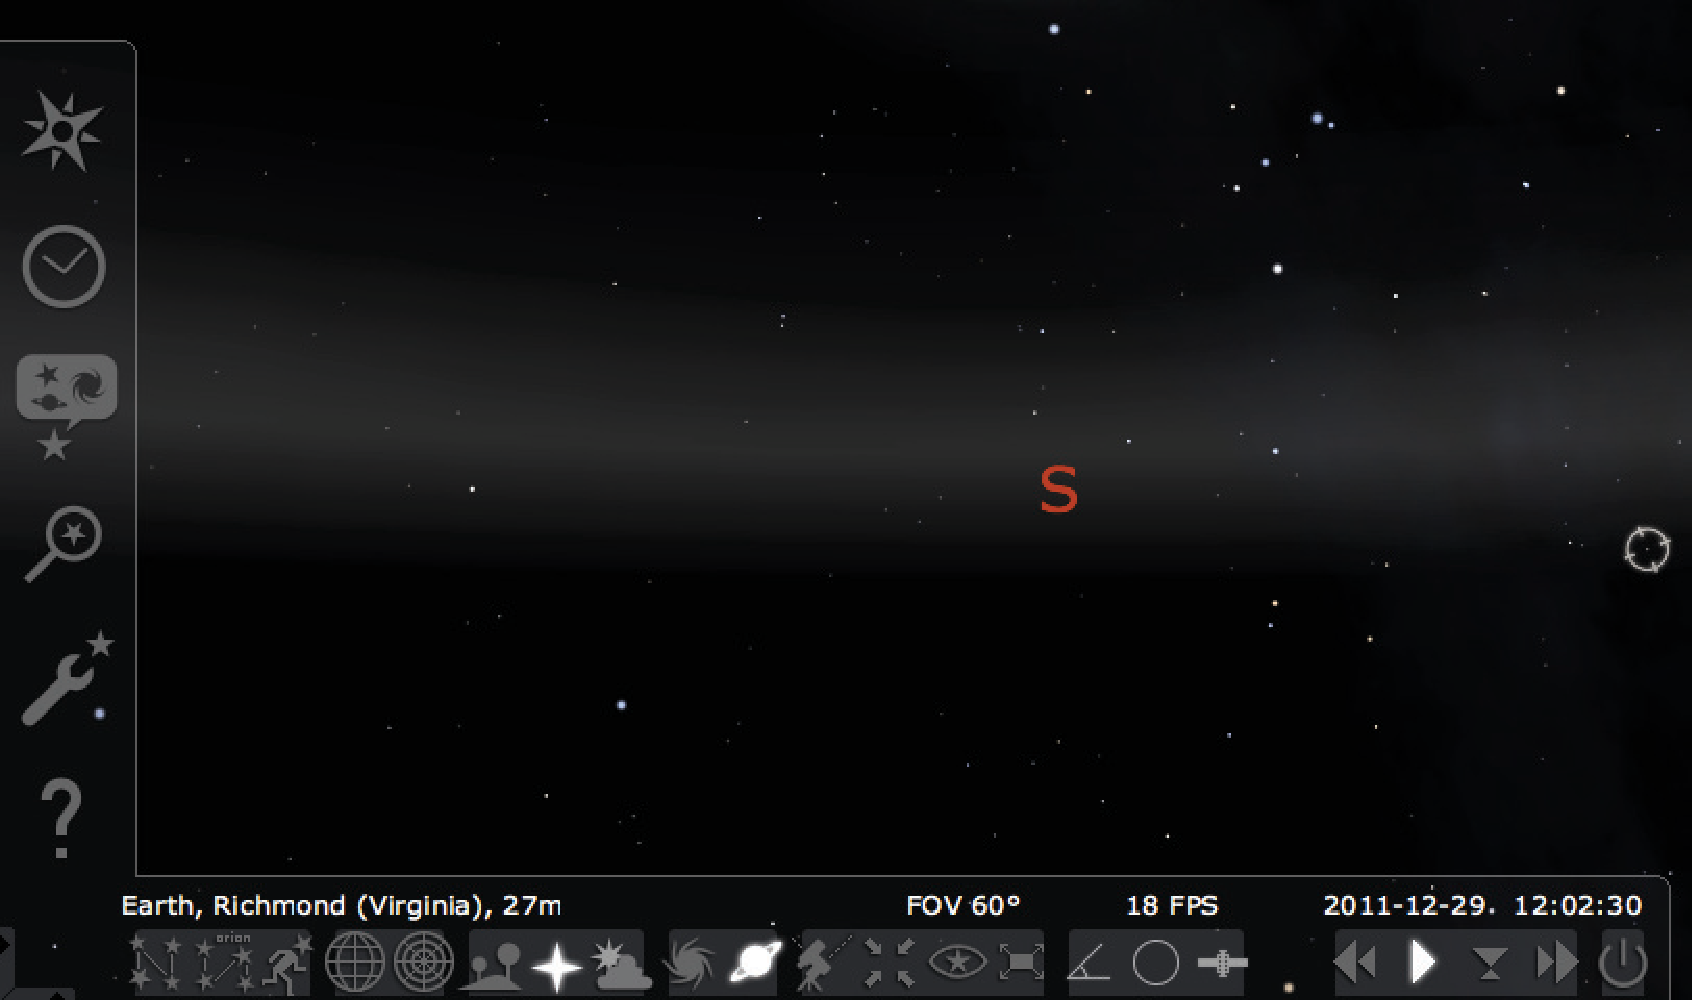
\includegraphics[width=4in]{appendices/stellarium/stellarium-icons.pdf}
\vspace{0.1in}
\end{center}

In the descriptions below, I'll refer quite a bit to
the various icons in these menus. 

\paragraph{Starting up and closing down the program.}
You start \stellarium\ in the usual way.
When you're done with the program, you exit by
clicking on this icon: \icon{exit}.

When you first start \textit{Stellarium}, position the mouse
near the bottom of the screen so that the horizontal
row of icons appears. You may find that the
Angle Measure icon \icon{angular} doesn't appear in this row.
If you're going to want to measure angular separations (which is
something we'll do pretty often), you'll need to fix this before proceeding.
Here's how. Click on the configuration icon \icon{config}, then click on
``Plugins.'' The words ``Angle Measure'' should be highlighted at the 
upper left of the configuration box. There's a checkbox at the bottom
of this box, next to the words ``Load at startup.'' Check this box.
Then exit \stellarium\ (\icon{exit}), and start it again.


\paragraph{Moving around the sky.} Hold down the left mouse button
(starting anywhere on the screen) and drag to look at different parts
of the sky.


\paragraph{Zooming in and out.} Use the mouse wheel or the page-up and 
page-down keys to
zoom in and out. Note that the ``Field of View'' (FOV) is indicated
at the bottom of the screen. The FOV is the size (in degrees) of the
patch of sky that's visible on the screen at that moment.

\paragraph{Selecting and centering on an object.}
If you click on a star or planet (or other celestial object), it will
be highlighted, and some (possibly cryptic) information on
the object will appear in the upper left corner. If you hit the
space bar or click on \icon{center}, that object will be moved to the
field of view.

\paragraph{Changing the observer's location.} Click on 
\icon{loc} to pull up a box that lets you
choose where the observer is located. You can either enter latitude
and longitude or choose a city from a list. You can even change your
observation location to the Moon or another planet.

\paragraph{Changing time.} There are two ways to adjust the 
time.

The first is to use these icons: 
\icon{time1}. These let you adjust
how fast time is flowing in the simulation.
The second icon is a play/pause button, which starts and stops the flow
of time. The ones on the left and right adjust the speed of the playback.
The third one resets the time to the present moment.

If you want to go to a specific moment in time, you're better off
using the clock icon, \icon{time2}. This causes a
box to pop up in which you can adjust the date and time to anything
you like. You can also use this box to jump forward in time by fixed
increments (one hour, one day, etc.)

\paragraph{Finding a specific object.} Click \icon{find}.

\paragraph{Miscellaneous display options.} 

These three icons help you identify
constellations: \icon{constellations}. The first draws lines connecting
the stars in each constellation. The second labels the constellations by
name. The third draws pictures of each constellation. (Personally, I
don't think the last one is much use.) All three of these are toggles --
that is, repeatedly clicking them flips the feature on and off.

Astronomers label points in the sky with two kinds of coordinates, equatorial
and azimuthal. (Note: \textit{Sky Safari} calls the latter
coordinate system ``horizon coordinates.'') 
We'll talk about these in detail in class,
but for the moment here are the basics.
Both of these are like latitude and longitude on Earth. The
difference is that the equatorial grid is ``attached'' to the sky, so
that each star's coordinates stay the same as time passes. The azimuthal 
grid, on the other hand, 
is attached to the Earth. You can turn on grids showing these two coordinate systems
using these icons: \icon{grids}.

The \icon{planets} icon turns on and off labels identifying the names of 
planets
and their moons.

The \icon{ground} icon switches the Earth's surface between being
solid and transparent. If you turn off the Earth's surface, you can
see objects even when they're below the horizon. 

The \icon{atmosphere} icon switches on and off the effects of 
Earth's atmosphere. When the atmosphere is ``turned off,'' you
can see the stars even in the daytime.

Of course, the last two represent things we can't do in real life
(no matter how much astronomers wish we could), but they're
useful tools for helping to build intuition about how
objects move in the sky.

\paragraph{Measuring angles.}
Often, we want to know the \textit{angular separation} between two
objects in the sky. Angular separation is the angle between a line from your eye
to one object and a line from your eye to the other object; it's a measure
of how far apart the objects appear to be. To determine
angular separation, click on the icon \icon{angular}, and then drag
the mouse (holding down the left button) from one object to the other.
When you're done measuring angles, click the \icon{angular} icon again.

\paragraph{Switching between equatorial and azimuthal mounts.}
As we'll see in detail, objects in the night sky appear to rotate
approximately once per day about a point in the sky called the ``north
celestial pole.'' This apparent motion is really due to the 
Earth's rotation on its axis. 
Often, it's useful to examine what the sky would look like if
the Earth's rotation could be taken away. Clicking on the 
\icon{mount} icon switches back and forth between two ways of looking
at the sky: the ``azimuthal'' view shows  the sky as it really looks from 
a given point on the surface of the rotating Earth, and the ``equatorial''
view shows
what happens when the Earth's rotation is taken away.

As a matter of fact, astronomical telescopes are often
placed on an ``equatorial mount,'' which has a motor that 
rotates the telescope
in just the right way to cancel out the Earth's motion. The 
equatorial point of view is what we actually see in this case.  

Note: These two types of ``mounts'' are what I called the
``stationary-Earth'' and ``stationary-sky'' points of view
in the \textit{Sky Safari} appendix. 
